%!Tex Program = lualatex
\documentclass[a4paper]{article}

\usepackage{lipsum}
\usepackage{graphicx}
\usepackage{subcaption}

% hyperlink
\usepackage{hyperref}
\hypersetup{
  colorlinks= true,  %Colours links instead of ugly boxes
  urlcolor  = blue,  %Colour for external hyperlinks
  linkcolor = black, %Colour of internal links
  citecolor = red    %Colour of citations
}

% compatibility issues
\usepackage{cprotect} % allow verbatim, etc., in macro arguments
\usepackage{float} % prevents things from floating everywhere
\usepackage{hypcap} % The package offers a solution to the problem that when you link to a float using hyperref, the link anchors to below the float's caption, rather than the beginning of the float.

% geometry
\usepackage{geometry}
\geometry{a4paper, scale=0.8, left=1in, right=1in, top=1in, bottom=1in}

% emoji
\usepackage{emoji}
\setemojifont{Twemoji Mozilla}
%\setemojifont{TwemojiMozilla.ttf}[Path=./]
%\newfontface\EmojiFont{Twemoji Mozilla}[Renderer=HarfBuzz]

\usepackage{amsmath}
\usepackage{amssymb}

% Headers & Footnotes
\usepackage{fancyhdr}
\lhead{Page \thepage}
\chead{}
\rhead{\LaTeXe{} Cheatsheet}
\lfoot{}
\cfoot{\thepage}
\rfoot{}
\renewcommand{\headrulewidth}{0.4pt}
\renewcommand{\footrulewidth}{0pt}
% Include \thispagestyle{firstpagestyle} immediately after \maketitle for first page styling
\fancypagestyle{firstpagestyle}{
	\fancyhf{}
	\cfoot{\thepage}
	\renewcommand{\headrulewidth}{0pt}
	\renewcommand{\footrulewidth}{0.4pt}
}

% TikZ & Python
\usepackage{tikz}
\usepackage{pythontex}

% 中文支持
\usepackage{luatexja-fontspec}
\setmainjfont{simkai}
\newjfontfamily{\song}{simsun}

% tables
\usepackage{csvsimple}
\usepackage{multicol}
\setlength\columnsep{15pt}
\usepackage{multirow}
\usepackage{booktabs}

% algorithms
\usepackage{minted}
\usemintedstyle{colorful}
\usepackage{algorithm}
\usepackage{algpseudocode}

% typesetting, others & trivials
\usepackage{fontspec}
%\setmainfont{Calibri}
%\renewcommand{\familydefault}{\sfdefault}
\newfontfamily\calibri{Calibri}
\setlength{\parindent}{0em} % paragraph indentation size
\setlength{\parskip}{0em} % space between paragraphs
\renewcommand{\baselinestretch}{1} % line spacing


% illustrate lua with circuitikz
\usepackage{luacode}
\usepackage{circuitikz}


% Math Operator
\DeclareMathOperator{\arctg}{arctg}
\renewcommand\x{\mathbf{x}}
\newcommand\y{\mathbf{y}}
\newcommand\W{\mathbf{W}}
\newcommand\R{\mathbb{R}}


\title{\LaTeXe{} Cheatsheet}
\author{Shaoming Zheng}
\date{December 32, 2021}

\begin{document}

\maketitle
\thispagestyle{firstpagestyle}

\tableofcontents

\begin{quote}
\begin{itemize}
\item Don't hesitate to read all sentences \& code of this doc. It answers most of the puzzles.
\item \LaTeX{} is a good regularization scheme to write academic works compared to MS Word and the de facto standard in academia. However, typesetting in \LaTeX{} is also terribly unrobust, highly mysterious, stubbornly unreasonable, confusing, counter-intuitive, complicated, hard-to-memorize, buggy yet undebuggable, packages-dependent, restrictive, and involves many obsolete programming fashions.
\item Therefore, this cheat sheet serves as a collection of common snippets in a common article (for a book you may need extra features such as indices \& glossaries etc.) and it would be a terrible typesetting experience if you don't have something similar in hand. It tries to support both aesthetics from designers' perspective and workflow conveniences from engineers' perspective while being as least hacky as possible. Most of them are self-explanatory for basic users.
\item However, it's still far from capturing all the subtleties of \LaTeX{}, e.g. hyperlinks. It will be frequently updated after I discovered more in everyday usages. To explore more of \LaTeX, I recommend the following resources:
\begin{itemize}
\item Documentation of packages: \href{https://ctan.org/}{CTAN}
\item Topics-organized tutorials: \href{https://www.overleaf.com/learn}{Overleaf}
\item General docs: \href{https://latexref.xyz/}{\LaTeXe{} unofficial reference manual}
\end{itemize}
\item Note that some of the usage (such as the geometry package) are only in the preamble. Please refer to the code with comments.
\item I recommend using Lua\LaTeX + \TeX{} Live + \TeX{} Studio (Windows), \TeX Pad (macOS), or Overleaf (for collab). 
\begin{itemize}
\item You might think that a more lightweight bundle such as \href{https://yihui.org/tinytex/}{Tiny\TeX{}} is preferrable, but you end up having to install packages every time you use a new template. 
\item Compared to popular versatile editor such as Visual Studio Code or IDEs, \TeX{} Studio, though ugly in interface, is dedicated to \TeX{} and contains many shortcuts.
\item Lua\LaTeX is the newest \TeX{} engine. It provides a new programming framework which some new features require.
\end{itemize}
\item When a .sty file is missing (especially if you're using Tiny\TeX{}), use \texttt{tlmgr search --global --file XX.sty} to find the package name. Then, use \texttt{tlmgr install YY.sty} (though YY is usually the same with XX). 对于国内用户,请换用清华源:\texttt{tlmgr option repository https://mirrors.tuna.tsinghua.edu.cn/CTAN/systems/texlive/tlnet
}
\end{itemize}
\end{quote}

\section{Mathematics}

\subsection{Equations}

\begin{equation}
	\binom{n}{k} = \frac{n!}{k!(n-k)!},\quad
	\arctg \frac{\pi}{3} = \sqrt{3},\quad
	\y = \x\W,\; \text{where}\; \x \in \R^{n\times m}, \W \in \R^{m\times 1}, \y \in \R^{n\times 1}
\end{equation}

\begin{align}
2x - 5y &=  8 \\ 
3x + 9y &=  -12
\end{align}

\begin{equation}
\int_{a}^{b} x^2 \,dx = \oint_V f(s) \,ds = \sum_{n=1}^{\infty} 2^{-n} = \prod_{i=a}^{b} f(i) = \lim_{x\to\infty} f(x) = 1
\end{equation}

For a list of greek letters and math symbols, please visit \href{https://www.overleaf.com/learn/latex/List_of_Greek_letters_and_math_symbols}{here}.

\subsection{Matrix}

\begin{equation}
A = \begin{bmatrix}
1 & 2 & 3\\
a & b & c
\end{bmatrix},\quad
\Sigma = \begin{bmatrix}
   \sigma_{11} & \sigma_{12} & \cdots & \sigma_{1n} \\
	 \sigma_{21} & \sigma_{22} & \cdots & \sigma_{2n} \\
   \vdots & \vdots & \ddots & \vdots \\
	 \sigma_{n1} & \sigma_{n2} & \cdots & \sigma_{nn}
\end{bmatrix}
\end{equation}

\subsection{Spacing}

\begin{equation}
S = \{ z \in \mathbb{C}\, |\, |z| < 1 \} \quad \textrm{and} \quad S_2=\partial{S}
\end{equation}

We can change the inline style from $\frac{1}{x+1}$ to $\displaystyle \frac{1}{x+1}$ by \verb|\displaystyle|.

\begin{figure}[H]
\centering
\begin{tabular}{l|l}
\hline
\LaTeX{} code &	Description \\
\hline
\verb|\quad| &	space equal to the current font size (= 18 mu) \\
\verb|\,| & 3/18 of \verb|\quad| (= 3 mu) \\
\verb|\:| & 4/18 of \verb|\quad| (= 4 mu) \\
\verb|\;| & 5/18 of \verb|\quad| (= 5 mu) \\
\verb|\!| & -3/18 of \verb|\quad| (= -3 mu) \\
\verb|\ |(space after backslasH) & equivalent of space in normal text \\
\verb|\qquad| & twice of \verb|\quad| (= 36 mu) \\
\hline
\end{tabular}
\end{figure}

\section{Figures}

\begin{figure}[H]
\centering
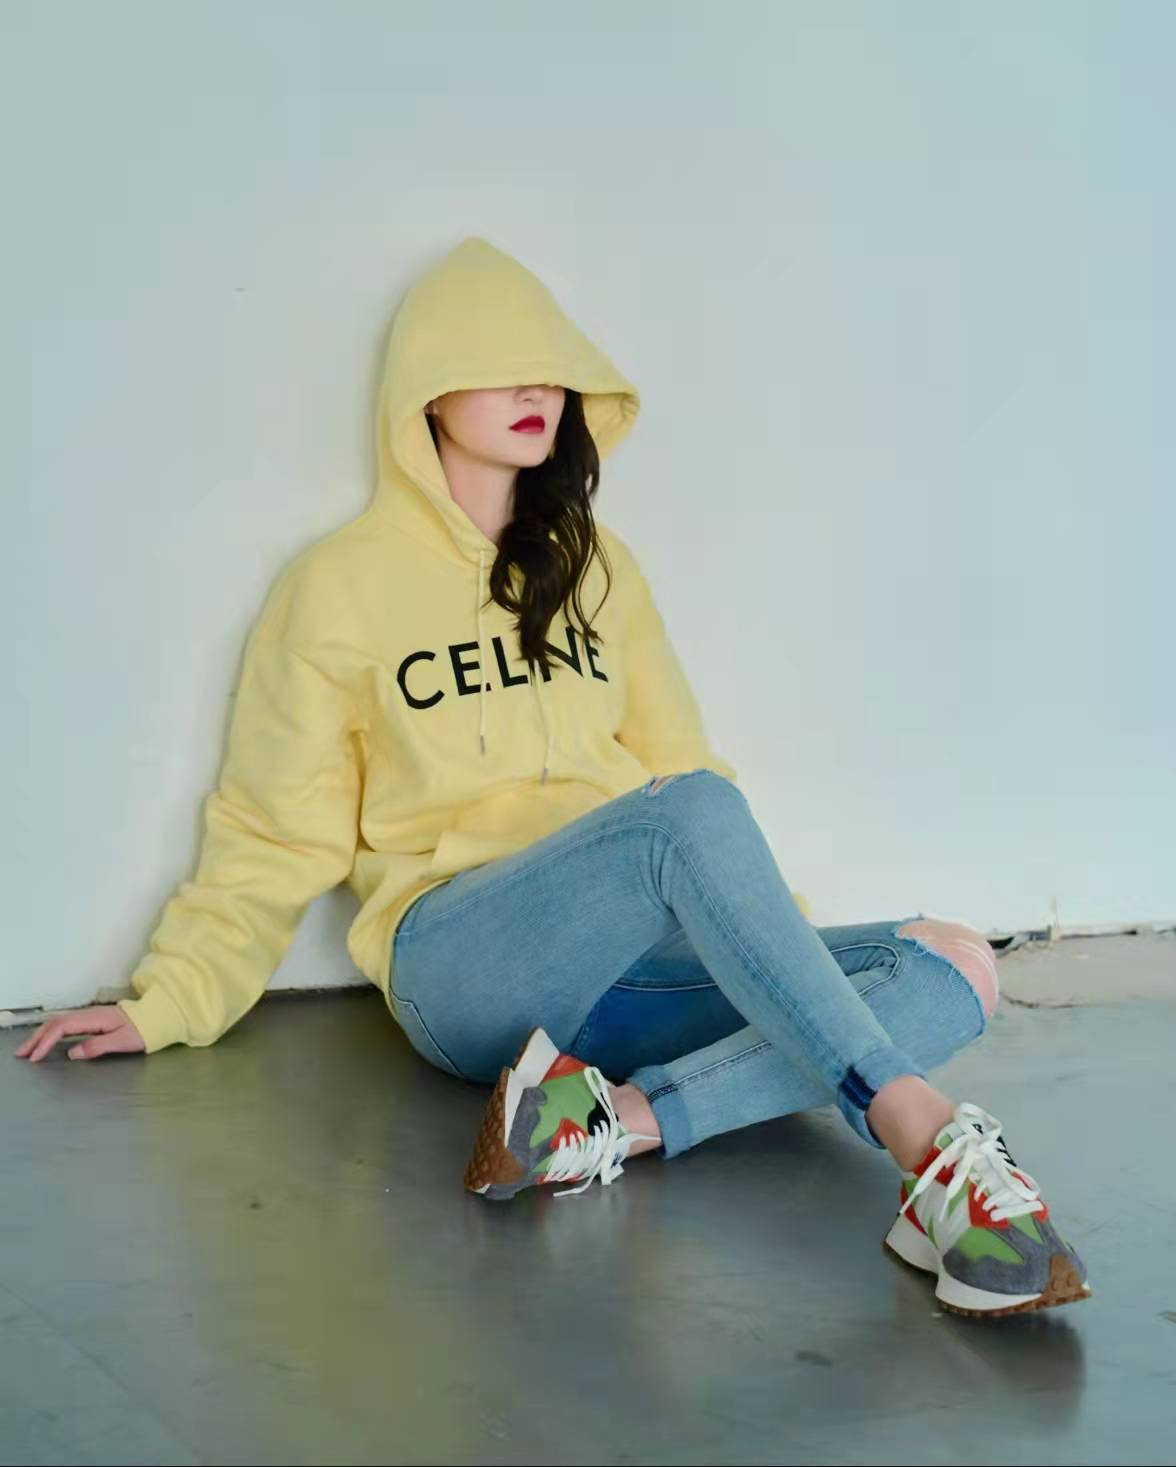
\includegraphics[width=0.4\linewidth]{images/lq0}
\caption{Example of a single figure}
\label{fig:example1}
\end{figure}

\begin{figure}[H]
	\centering
	\begin{subfigure}{0.365\linewidth}
		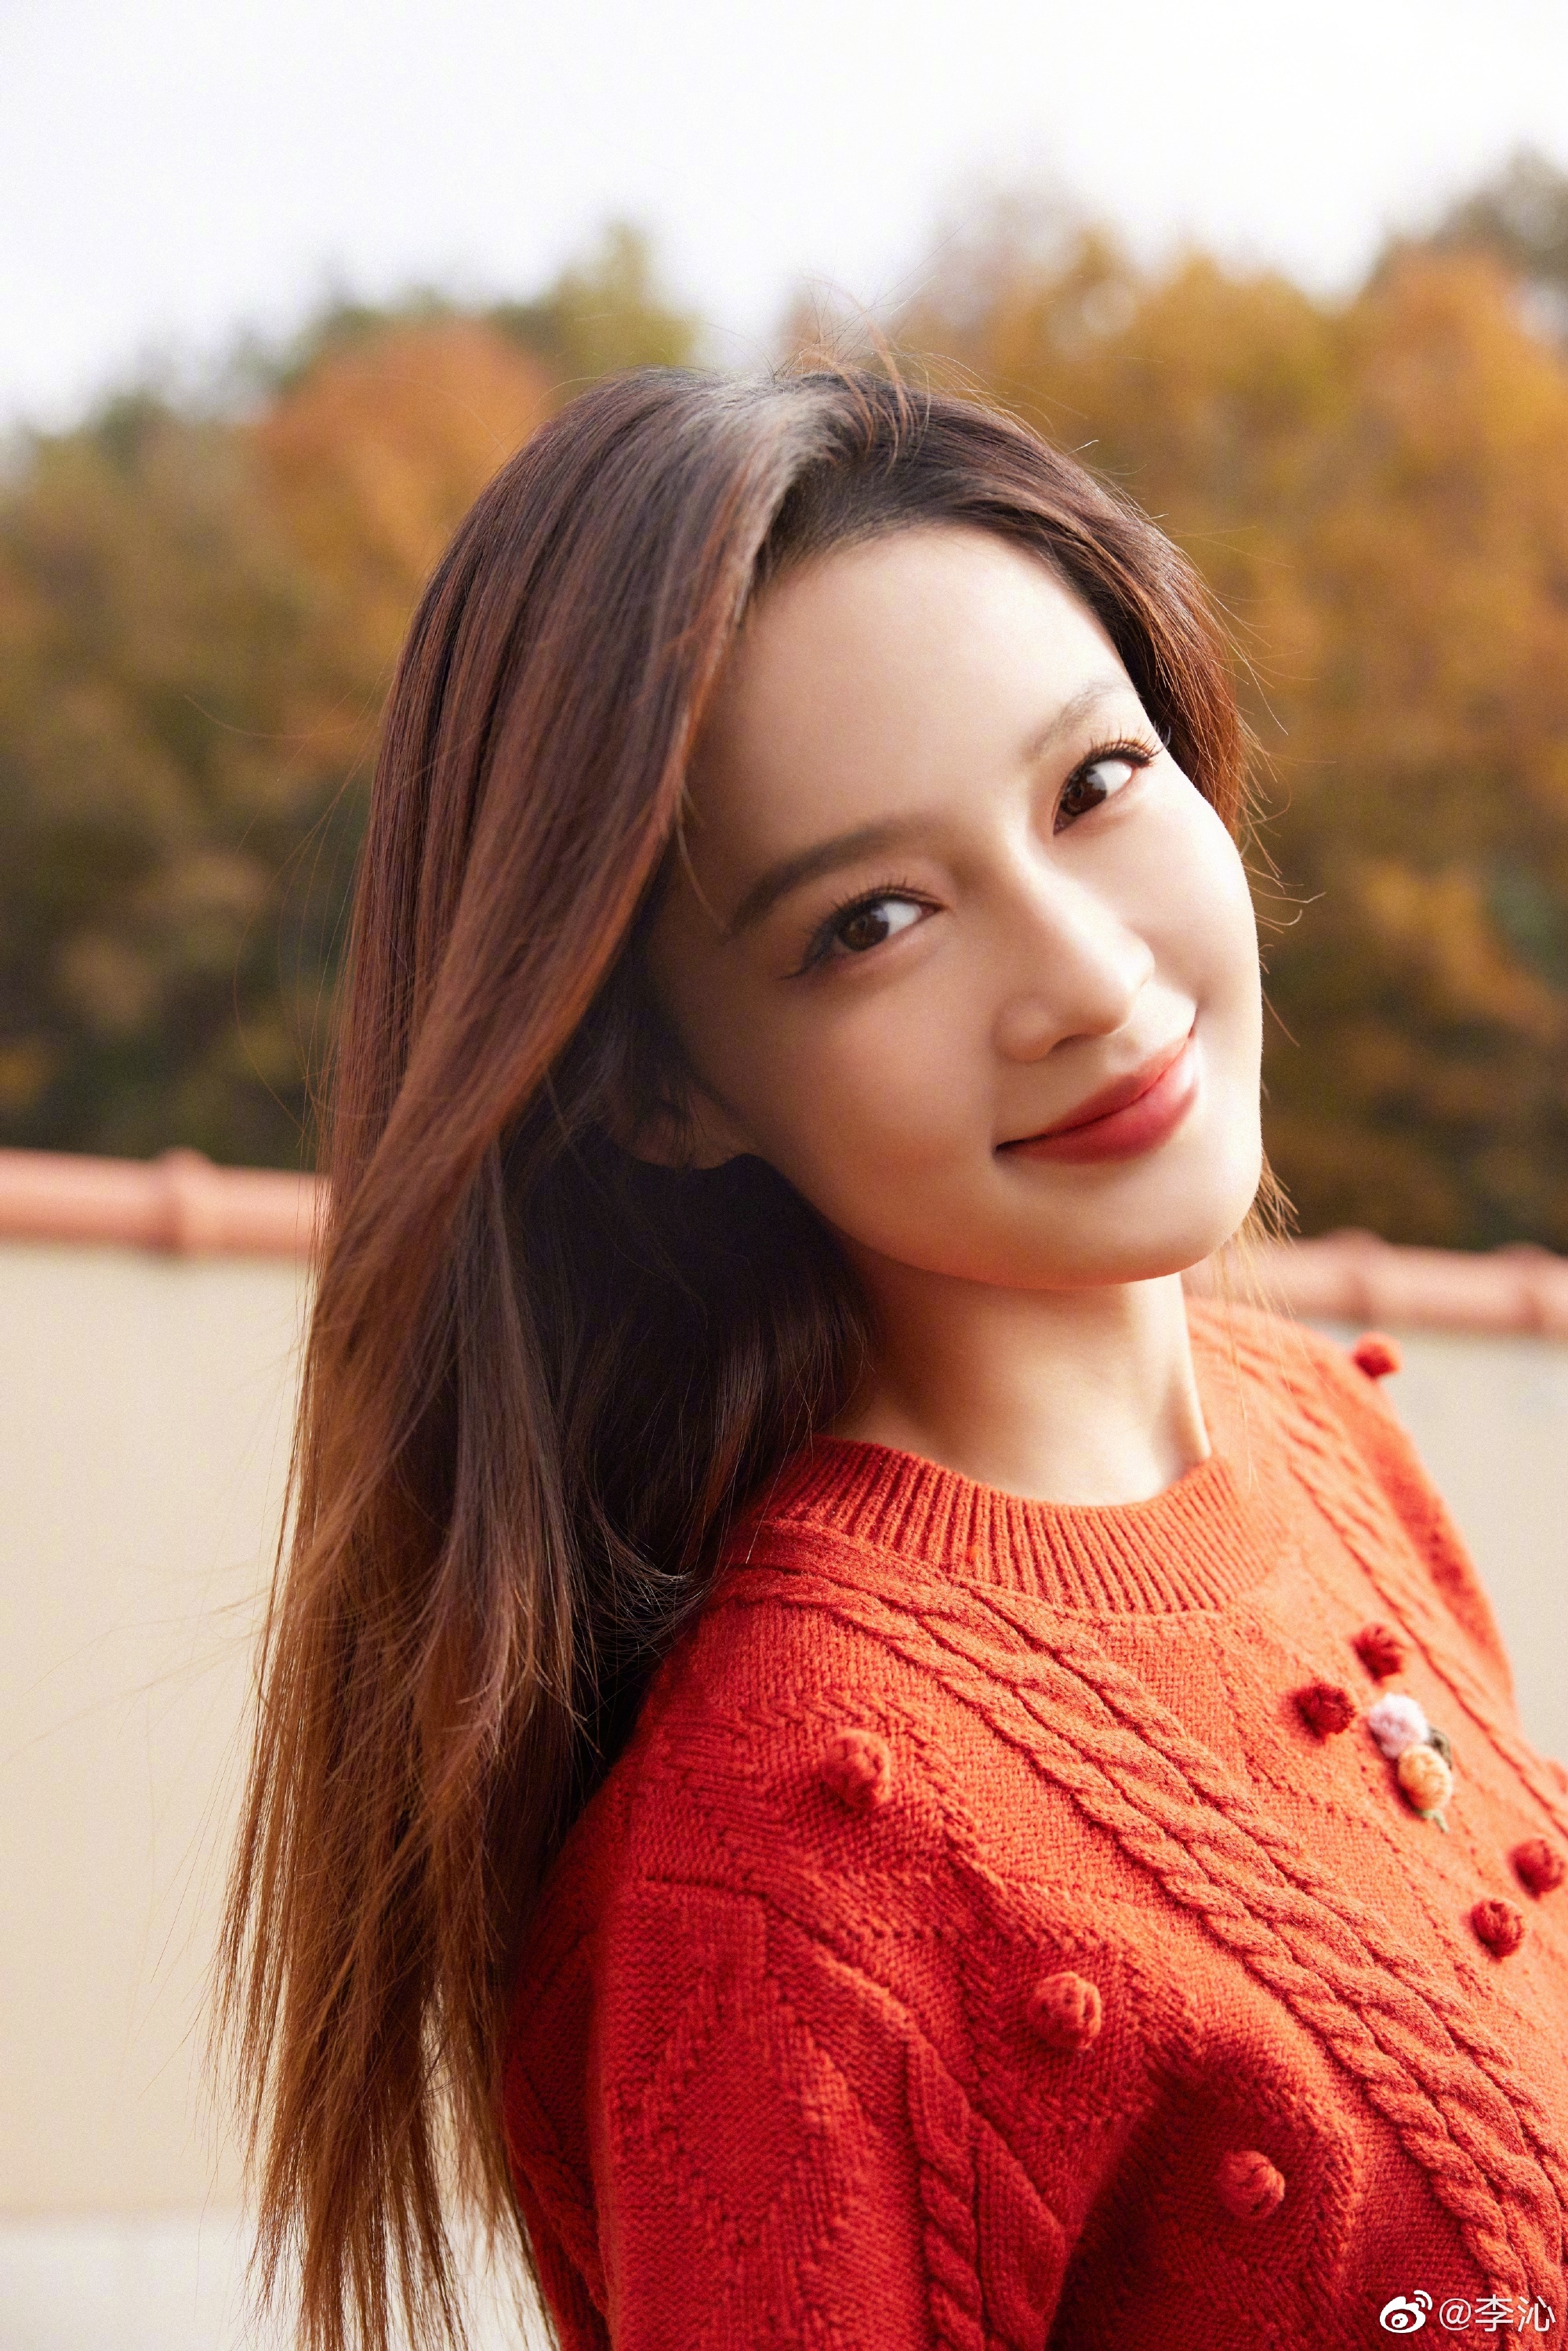
\includegraphics[width=\linewidth]{images/lq1}
		\caption{\emoji{heart-eyes}}
	\end{subfigure}
	\begin{subfigure}{0.4\linewidth}
		
\includegraphics[width=\linewidth]{images/lq2}
		\begin{subfigure}{0.49\linewidth}
			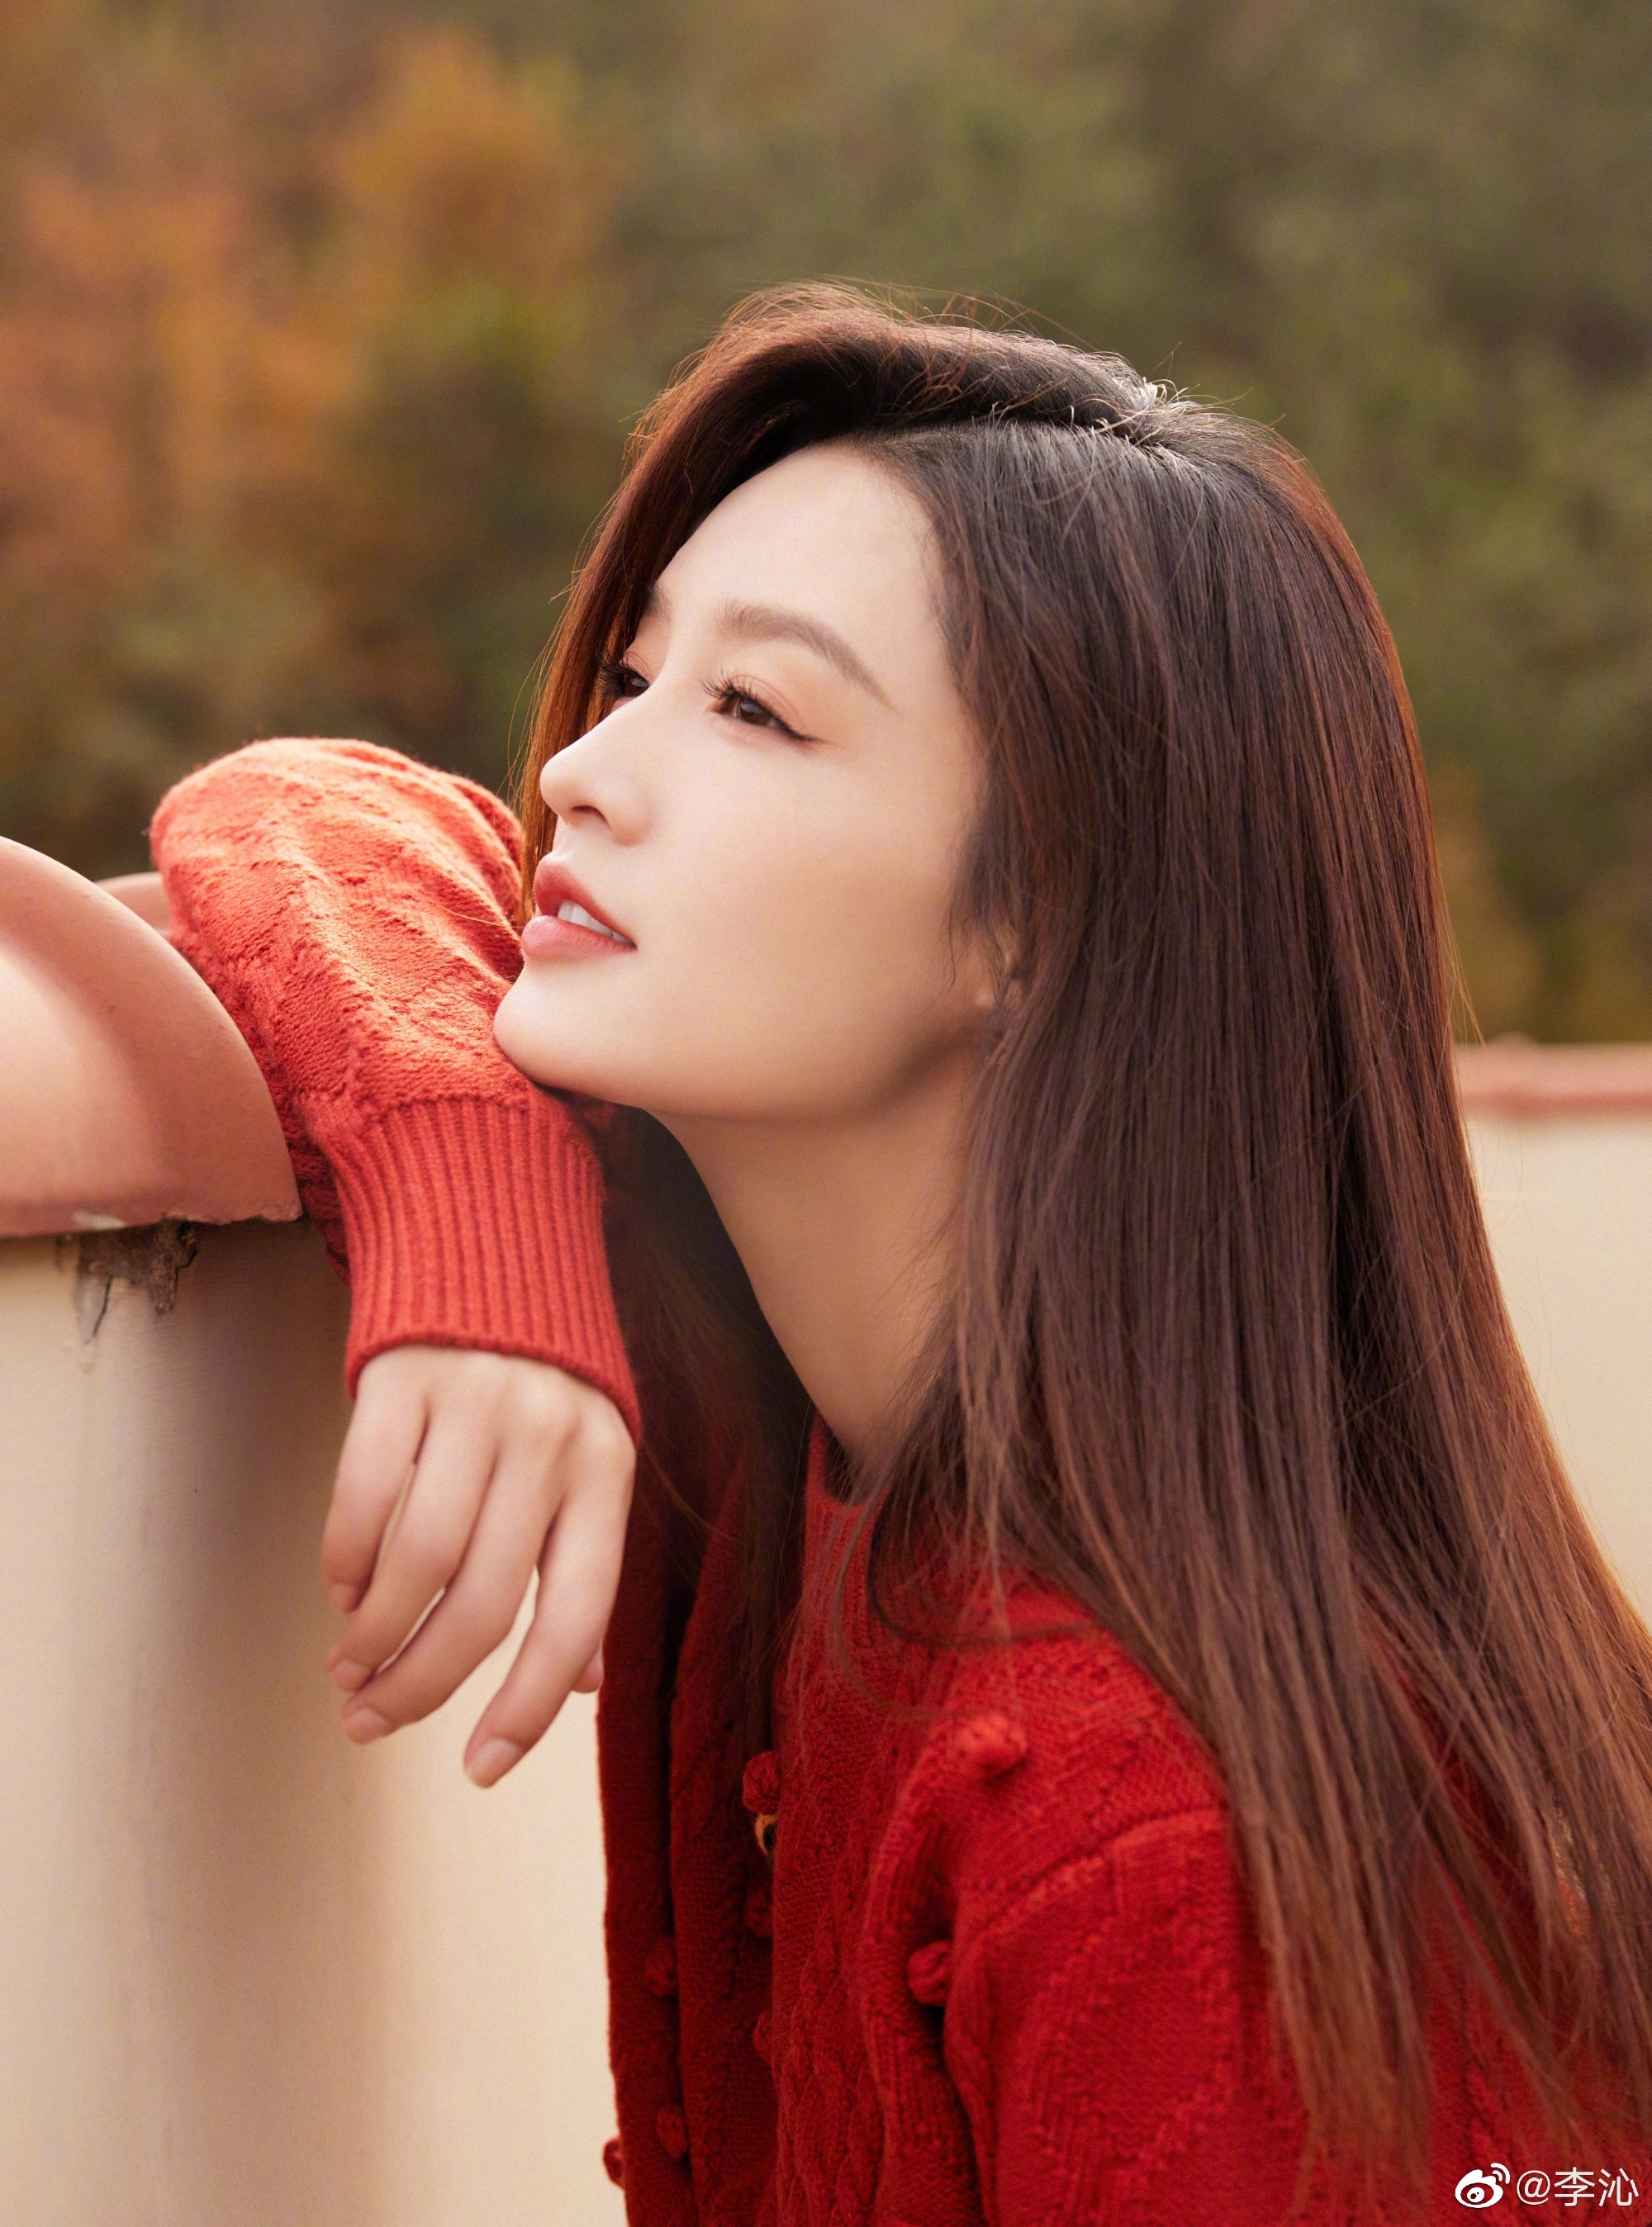
\includegraphics[width=\linewidth]{images/lq3}
			\caption{\emoji{kissing-heart}}
		\end{subfigure}
		\begin{subfigure}{0.49\linewidth}
			
\includegraphics[width=\linewidth]{images/lq4}
			\caption{\emoji{revolving-hearts}}
		\end{subfigure}
	\end{subfigure}
	
	\cprotect\caption{Example of nested subfigures controlled by \verb|\linewidth|}
	\label{fig:example2}
\end{figure}

Please use \texttt{[H]} to position most figures. I would like to refer to Figure \ref{fig:example1}. You can directly paste an image into \TeX{} Studio. When you link to a float using hyperref, the link anchors to below the float's caption. To anchor to the beginning of the float, insert a \verb|\capstart| in the beginning.

\section{Tables}
We appreciate building tables from external files (csv).

\begin{table}[H]
\setlength{\tabcolsep}{1.5 mm}
\caption{Example of CSV-generated metrics evaluation table}
\centering
\begin{tabular}{lp{2cm}p{2cm}p{2cm}p{2cm}p{2cm}}
  \toprule[1pt]
	\multirow{2}{*}{Methods} & \multicolumn{2}{c}{Category I} & \multicolumn{2}{c}{Category II} \\
  \cmidrule(lr){2-3} \cmidrule(lr){4-5}
	& Metric Ia $\uparrow$ & Metric Ib$\uparrow$ & Metric IIa $\downarrow$ & Metric IIb $\uparrow$ \\
	\cmidrule(lr){1-3} \cmidrule(lr){4-5}
	\csvreader[
		head to column names,
		late after line=\\,
		late after last line=\\\cmidrule(lr){1-3} \cmidrule(lr){4-5}
	]{tables/table1.csv}{}{\method & \a & \b & \c & \d}
	\textbf{Ours} & \textbf{.123}(.456) & \textbf{.123}(.456) & \textbf{.123}(.456) & .123(.456) \\
	\bottomrule[1pt]
\end{tabular}
\label{table:table1}
\end{table}

\begin{table}[H]
	\centering
	\caption{Example of a minimalist trilinear table}
	\begin{tabular}{c|c|c}
		\hline
	  a & b & c \\\hline
		1 & 2 & 3 \\
		1 & 2 & 3 \\\hline
	\end{tabular}
\end{table}

\noindent
Besides, there is a helpful \href{https://www.tablesgenerator.com/}{tool} for creating tables.

\section{Algorithms}

\subsection{Pseudocode (also showing multi-column \& local fonts)}

\begin{multicols}{2}
If you want a figure to span 2 columns in a two-column document, use star with relative positioning \verb|\begin{table*}[t]|
{\calibri \small \lipsum[1]}
\begin{algorithm}[H]
\centering
\caption{An algorithm with caption}\label{alg:cap}
\begin{algorithmic}[1]
\Require $n \geq 0$
\Ensure $y = x^n$
\State $y \gets 1$
\State $X \gets x$
\State $N \gets n$
\While{$N \neq 0$}
\If{$N$ is even}
    \State $X \gets X \times X$
    \State $N \gets \frac{N}{2}$  \Comment{This is a comment}
\ElsIf{$N$ is odd}
    \State $y \gets y \times X$
    \State $N \gets N - 1$
\EndIf
\EndWhile
\end{algorithmic}
\end{algorithm}
\end{multicols}

\subsection{Code}

To use \texttt{minted}, you need to add the \texttt{--escape-shell} flag to the \texttt{lualatex} command and install \texttt{pygmentize} for Python. Sometimes, it can't find you \texttt{pygmentize}, you'll need to add your \texttt{pygmentize} to the front of your PATH. Here, we would like to let minted directly import a Python file.
\inputminted[linenos]{python}{code/code1.py}
Otherwise, we can use \verb|\begin{minted}[linos]{python}...\end{minted}| instead. You can also use minted inline: \mintinline{python}{print(x**2)}. You can change the color scheme via \verb|\usemintedstyle{<name>}|, and preview all the available schemes \href{https://pygments.org/styles/}{here}.

\section{Fonts}

\subsection{中文支持}

这是(楷体)中文,需要调用\verb|luatexja-fontspec|包并\verb|\setjmainfont(simkai)|。注意\verb|simkai|为字体文件(\verb|simkai.ttf|)名而非字体名(``楷体")。{\song 通过\verb|\newjfontfamily|,也可以局部使用新字体。}更多用法参见\href{https://ctan.math.utah.edu/ctan/tex-archive/macros/luatex/generic/luatexja/doc/luatexja-en.pdf}{luatexja包文档}。\\

\subsection{Emoji}
For the list of supported emoji aliases, visit \href{https://ctan.math.utah.edu/ctan/tex-archive/macros/luatex/latex/emoji/emoji-doc.pdf}{emoji package docs}. Note that this feature is highly unstable and only (indeterministically) some aliases are supported.
\begin{equation}
\log \text{\emoji{sweat-smile}} = \text{\emoji{droplet}} \log \text{\emoji{smile}}
\end{equation}

\section{TikZ \& Python}

% \begin{pycode}
from math import sin, cos, pi

R1 = 0.7
R2 = 2
R3 = 3/8 * (R2 - R1)
coord = lambda R, a: (R * cos(a), R * sin(a))
\end{pycode}
		
\begin{figure}[H]
\capstart
\centering
\begin{tikzpicture}[scale=2]
	% colors
	\colorlet{a1a2}{cyan}
	\colorlet{a3}{violet}
	\colorlet{dex}{magenta}
	\colorlet{end}{red}
	
	% styles
	\tikzstyle{info box}=[rounded corners,fill=red!10,inner sep=2ex]
	
	% link1 + link2 reachable workspace
	\begin{scope}
		\py{f'\draw[a1a2,fill=a1a2!15,even odd rule] (0,0) circle ({R2}) circle ({R1});'}
		\py{f'\draw[a1a2,->] (0,0) -- {coord(R1,pi/8)} node[above] {"{$|a_1 - a_2|$}"};'}
		\py{f'\draw[a1a2,->] (0,0) -- {coord(R2,-pi/4)} node[below] {"{$a_1 + a_2$}"};'}
	\end{scope}

	% dexterous workspace
	\begin{scope}
		\py{f'\draw[dex,fill=dex!15,opacity=0.8,even odd rule] (0,0) circle ({R2-R3}) circle ({R1+R3});'}
		\py{f'\draw[dex,->] (0,0) -- {coord(R1+R3,7*pi/8)} node[above] {"{$|a_1 - a_2| + a_3$}"};'}
		\py{f'\draw[dex,->] (0,0) -- {coord(R2-R3,5*pi/8)} node[above] {"{$a_1 + a_2 - a_3$}"};'}
	\end{scope}

	% last joint circles
	\begin{scope}
		\py{f'\coordinate (c1) at {coord(R1+R3,-3*pi/4)};'}
		\py{f'\draw[a3] (c1) circle ({R3});'}
		\py{f'\draw[fill=end] (c1) circle (0.04);'}
		\py{f'\draw[a3,->] (c1) -- {coord(R1,-3*pi/4)} node[above] {"{$a_3$}"};'}
	\end{scope}
	
	\begin{scope}
		\py{f'\coordinate (c2) at {coord(R2-R3,-pi/2)};'}
		\py{f'\draw[a3] (c2) circle ({R3});'}
		\py{f'\draw[fill=end] (c2) circle (0.04);'}
		\py{f'\draw[a3,->] (c2) -- {coord(R2,-pi/2)} node[below] {"{$a_3$}"};'}
	\end{scope}
				
	% coordinate frames
	\begin{scope}
		\draw[->] (0,0) -- (0.25,0) node[right] {$x_0$};
		\draw[->] (0,0) -- (0,0.25) node[above] {$y_0$};
	\end{scope}

	% text
	\draw[xshift=70] node [right,text width=7cm,style=info box]
	{
		{\color{dex}Dexterous workspace of the arm} is the region of end effectors. If we want the last joint to point to the end effector from any direction, the {\color{a3}possible locations of the last joint} (i.e. the {\color{a3}violet circle} with radius $a_3$ centered at the {\color{end}end effector}, two of which Figure \ref{fig:1} show as the extreme cases) should be \textit{fully included} in the {\color{a1a2}reachable workspace of link 1 + link 2}. The dexterous workspace therefore should be a ring with inner radius $|a_1 - a_2| + a_3$ and outer radius $a_1 + a_2 - a_3$ \textit{provided that} $a_1 + a_2 - a_3 \geq |a_1 - a_2| + a_3$, i.e. $a_3 \leq (a_1 + a_2 - |a_1 - a_2|) / 2$.
	};
\end{tikzpicture}
\caption{Dexterous workspace: $a_3 \leq (a_1 + a_2 - |a_1 - a_2|) / 2$} 
\label{fig:1}
\end{figure}
\begin{pycode}
from math import sin, cos, pi

R1 = 0.7
R2 = 2
R3 = 3/8 * (R2 - R1)
coord = lambda R, a: (R * cos(a), R * sin(a))
\end{pycode}
		
\begin{figure}[H]
\capstart
\centering
\begin{tikzpicture}[scale=2]
	% colors
	\colorlet{a1a2}{cyan}
	\colorlet{a3}{violet}
	\colorlet{dex}{magenta}
	\colorlet{end}{red}
	
	% styles
	\tikzstyle{info box}=[rounded corners,fill=red!10,inner sep=2ex]
	
	% link1 + link2 reachable workspace
	\begin{scope}
		\py{f'\draw[a1a2,fill=a1a2!15,even odd rule] (0,0) circle ({R2}) circle ({R1});'}
		\py{f'\draw[a1a2,->] (0,0) -- {coord(R1,pi/8)} node[above] {"{$|a_1 - a_2|$}"};'}
		\py{f'\draw[a1a2,->] (0,0) -- {coord(R2,-pi/4)} node[below] {"{$a_1 + a_2$}"};'}
	\end{scope}

	% dexterous workspace
	\begin{scope}
		\py{f'\draw[dex,fill=dex!15,opacity=0.8,even odd rule] (0,0) circle ({R2-R3}) circle ({R1+R3});'}
		\py{f'\draw[dex,->] (0,0) -- {coord(R1+R3,7*pi/8)} node[above] {"{$|a_1 - a_2| + a_3$}"};'}
		\py{f'\draw[dex,->] (0,0) -- {coord(R2-R3,5*pi/8)} node[above] {"{$a_1 + a_2 - a_3$}"};'}
	\end{scope}

	% last joint circles
	\begin{scope}
		\py{f'\coordinate (c1) at {coord(R1+R3,-3*pi/4)};'}
		\py{f'\draw[a3] (c1) circle ({R3});'}
		\py{f'\draw[fill=end] (c1) circle (0.04);'}
		\py{f'\draw[a3,->] (c1) -- {coord(R1,-3*pi/4)} node[above] {"{$a_3$}"};'}
	\end{scope}
	
	\begin{scope}
		\py{f'\coordinate (c2) at {coord(R2-R3,-pi/2)};'}
		\py{f'\draw[a3] (c2) circle ({R3});'}
		\py{f'\draw[fill=end] (c2) circle (0.04);'}
		\py{f'\draw[a3,->] (c2) -- {coord(R2,-pi/2)} node[below] {"{$a_3$}"};'}
	\end{scope}
				
	% coordinate frames
	\begin{scope}
		\draw[->] (0,0) -- (0.25,0) node[right] {$x_0$};
		\draw[->] (0,0) -- (0,0.25) node[above] {$y_0$};
	\end{scope}

	% text
	\draw[xshift=70] node [right,text width=7cm,style=info box]
	{
		{\color{dex}Dexterous workspace of the arm} is the region of end effectors. If we want the last joint to point to the end effector from any direction, the {\color{a3}possible locations of the last joint} (i.e. the {\color{a3}violet circle} with radius $a_3$ centered at the {\color{end}end effector}, two of which Figure \ref{fig:tikz} show as the extreme cases) should be \textit{fully included} in the {\color{a1a2}reachable workspace of link 1 + link 2}. The dexterous workspace therefore should be a ring with inner radius $|a_1 - a_2| + a_3$ and outer radius $a_1 + a_2 - a_3$ \textit{provided that} $a_1 + a_2 - a_3 \geq |a_1 - a_2| + a_3$, i.e. $a_3 \leq (a_1 + a_2 - |a_1 - a_2|) / 2$.
	};
\end{tikzpicture}
\caption{Dexterous workspace: $a_3 \leq (a_1 + a_2 - |a_1 - a_2|) / 2$} 
\label{fig:tikz}
\end{figure}

If you use python\TeX, you need to do a manual compilation of \texttt{pythontex XX.tex} between two \texttt{txs://lualatex}. For a detailed tutorials on python\TeX{} directives, visit \href{https://ctan.math.illinois.edu/macros/latex/contrib/pythontex/pythontex.pdf}{here}. Note that if you migrate TikZ to an external .tex file, it will occupy a whole page.

\section{Lua Programming with Domain Examples}

Lua is helpful in procedural typesetting via storing variables etc.

\luaexec{
tp=tex.print
local R1 = 0.1
local X1 = 0.3
local R2 = 0.13
local X2 = 0.35
local RC = 100
local XM = 40
tp("\\begin{figure}[H]")
tp("\\centering")
tp("\\begin{circuitikz}")
tp("\\draw (0,0) to[short,*-*] (10.5,0);")
tp("\\draw (0,4) to[short,*-,i=$I_1$] (1,4);")
tp("\\draw (1,4) to[R,l=$"..R1.."\\Omega$] (3,4);")
tp("\\draw (3,4) to[L,l=j$"..X1.."\\Omega$] (5,4);")
tp("\\draw (5,4) to[short] (5.5,4);")
tp("\\draw (5.5,4) to[L,l=j$"..X2.."\\Omega$] (7.5,4);")
tp("\\draw (7.5,4) to[R,l=$"..R2.."\\Omega$] (9.5,4);")
tp("\\draw (9.5,4) to[short,-*,i=$I_2'$] (10.5,4);")
tp("\\draw (5.25,4) to[short,*-*,,i=$I_0$] (5.25,3);")
tp("\\draw (5.25,3) to[short] (4.5,3)to [short] (4.5,2.75);")
tp("\\draw (5.25,3) to[short] (6,3) to [short] (6,2.75);")
tp("\\draw (4.5,2.75) to[R,l=$"..RC.."\\Omega$] (4.5,1.65);")
tp("\\draw (6,2.75) to[L,l=j$"..XM.."\\Omega$] (6,1.65);")
tp("\\draw (4.5,1.65) to[short] (4.5,1.4);")
tp("\\draw (6,1.65) to[short] (6,1.4) to [short] (4.5,1.4);")
tp("\\draw (5.25,1.4) to[short,*-*] (5.25,0);")
tp("\\draw (0,4) to [open,v=$V_1$] (0,0);")
tp("\\draw (10.5,4) to [open,v^=$V_2'$] (10.5,0);")
tp("\\end{circuitikz}")
tp("\\caption{One-phase transformer equivalent circuit (T-circuit)}")
tp("\\end{figure}")
}

\section{Others, Trivials \& General Troubleshooting}
\noindent
This is a sentence from \texttt{part1.tex}, which is different from \verb|\include{filename}|, where it does a \verb|\clearpage| first.
This is a footnote \footnote{foo bar}.\\
\begin{description}
\item[label] this is a description.
\end{description}
\begin{itemize}
\item Sometimes, you need to run \texttt{Build \& View} multiple times for somthing to show.
\item Sometimes, you need to delete all intermediate files (the ones recently created) if you're stuck in some error messages. Unfortunately, most \LaTeX error messages are not meaningful in any senses.
\item Sometimes, the loading order of \LaTeX{} packages are important. Observe the errors carefully to debug.
\end{itemize}


\section{Bibliography}

\begin{enumerate}
\item Put \href{https://www.ctan.org/tex-archive/biblio/bibtex/contrib/IEEEtran/IEEEtran.bst}{IEEEtran.bst} under the current directory.
\item Create a folder for my current article in Zotero.
\item Use Google Scholar to find an article.
\item Open the specific page and ``Save to Zotero'' into that folder (by default).
\item Right-click on the folder and export to BibTeX format, save the \texttt{.bib} file in the same directory of the article.
\item \texttt{Tools > Bibliography} and then \texttt{Build \& View}

This refers to an article \cite{li_cutpaste_2021}. And another one \cite{yang_learning_2021}.
\end{enumerate}

\bibliography{sample}
\bibliographystyle{IEEEtran}

\end{document}